\section{Introduction}
Generalised Parton Distributions (GPDs)
\cite{Mue94,Ji97,Rad97} encompass the familiar Parton
Distribution Functions (PDFs) and nucleon Form Factors (FFs) to provide a
comprehensive description of the structure of the nucleon. A thorough
description of the nucleon in terms of GPDs would allow the deduction
of the total angular momentum of partons in the nucleon, and the
construction of a longitudinal-momentum-dissected transverse spatial map of parton densities~\cite{Bur00}. The GPDs appear in experimental measurements in the form of complex-valued Compton Form Factors (CFFs), which are flavour-sums of convolutions of GPDs with hard scattering kernels. Constraints on these CFFs, and thus GPDs, can be obtained from measurements of exclusive \red{leptoproduction} processes. In particular, the exclusive leptoproduction of \red{a single} real photon from a nucleon or nucleus \red{that remains intact} ($e\,N\,\rightarrow\,e\,N\,\gamma$; see figure~\ref{spin}) is the simplest to describe and is the most widely-used reaction channel for such work (see \cite{Air01,Air06,Air08,Air09,Air10,Air10a,Air10b,Air11,Air11a,h101,h105,h107,h109,zeu03,zeu08,Maz07,Cam06,Ste01,Che06,Gir08,Gav09,Com10}).

Generalised parton distributions depend upon four kinematic variables: the
Mandelstam variable $t=(p-p^{\prime})^2$, which is the squared momentum
transfer to the target nucleon in the exclusive scattering process with $p$ ($p^{\prime}$)
representing the initial (final) four-momentum of the nucleon; the average
fraction $x$ of the nucleon's longitudinal momentum carried by the active
quark throughout the scattering process; half the difference of
  the fractions of the nucleon's longitudinal momentum carried
by the active quark at the start and end of the process, written as
the skewness $\xi$; and $Q^2=-(q^2)$, i.e. the negative square of the four-momentum of
the virtual photon that mediates the lepton-nucleon scattering
process. In the Bjorken limit of $Q^2\rightarrow\infty$ with fixed
$t$, the skewness $\xi$ is related to the Bjorken variable
$x_{\textrm{B}}=\frac{-q^2}{2p\cdot q}$ as
$\xi\approx\frac{x_\textrm{B}}{2-x_\textrm{B}}$. The results are presented
as a function of $x_{\textrm{B}}$ because there is no consensus on an experimentally observable representation of $\xi$. 
Exclusive leptoproduction of real photons
 arises from
two experimentally indistinguishable processes: the Deeply Virtual Compton Scattering (DVCS) process,
which is the emission of a real photon by the struck quark from the nucleon, and the Bethe--Heitler (BH) process, which is elastic lepton-nucleon scattering with the emission of a bremsstrahlung photon by the lepton.
\begin{figure}
\begin{center}
\subfigure[DVCS]{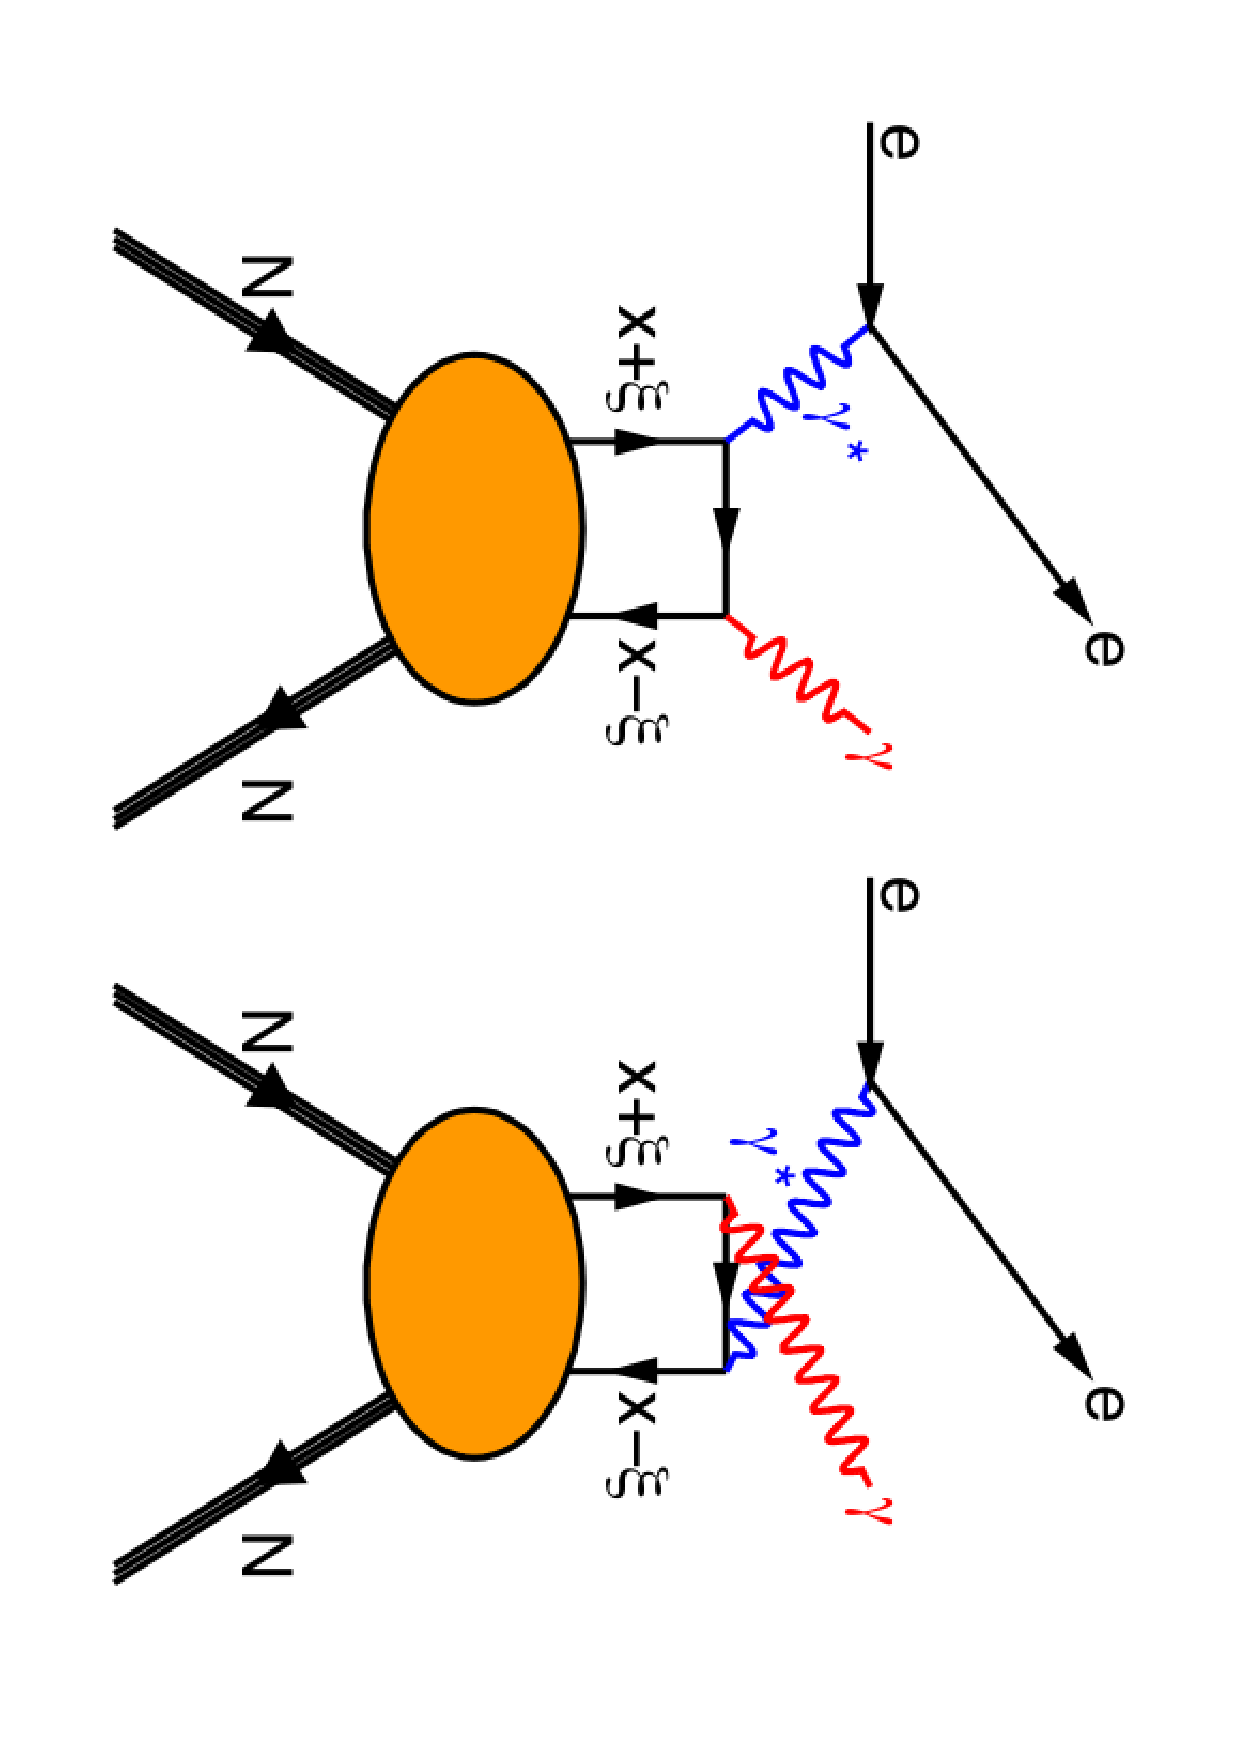
\includegraphics[angle=90,width=0.45\textwidth]{dvcs_both_edited}}
\subfigure[Bethe-Heitler]{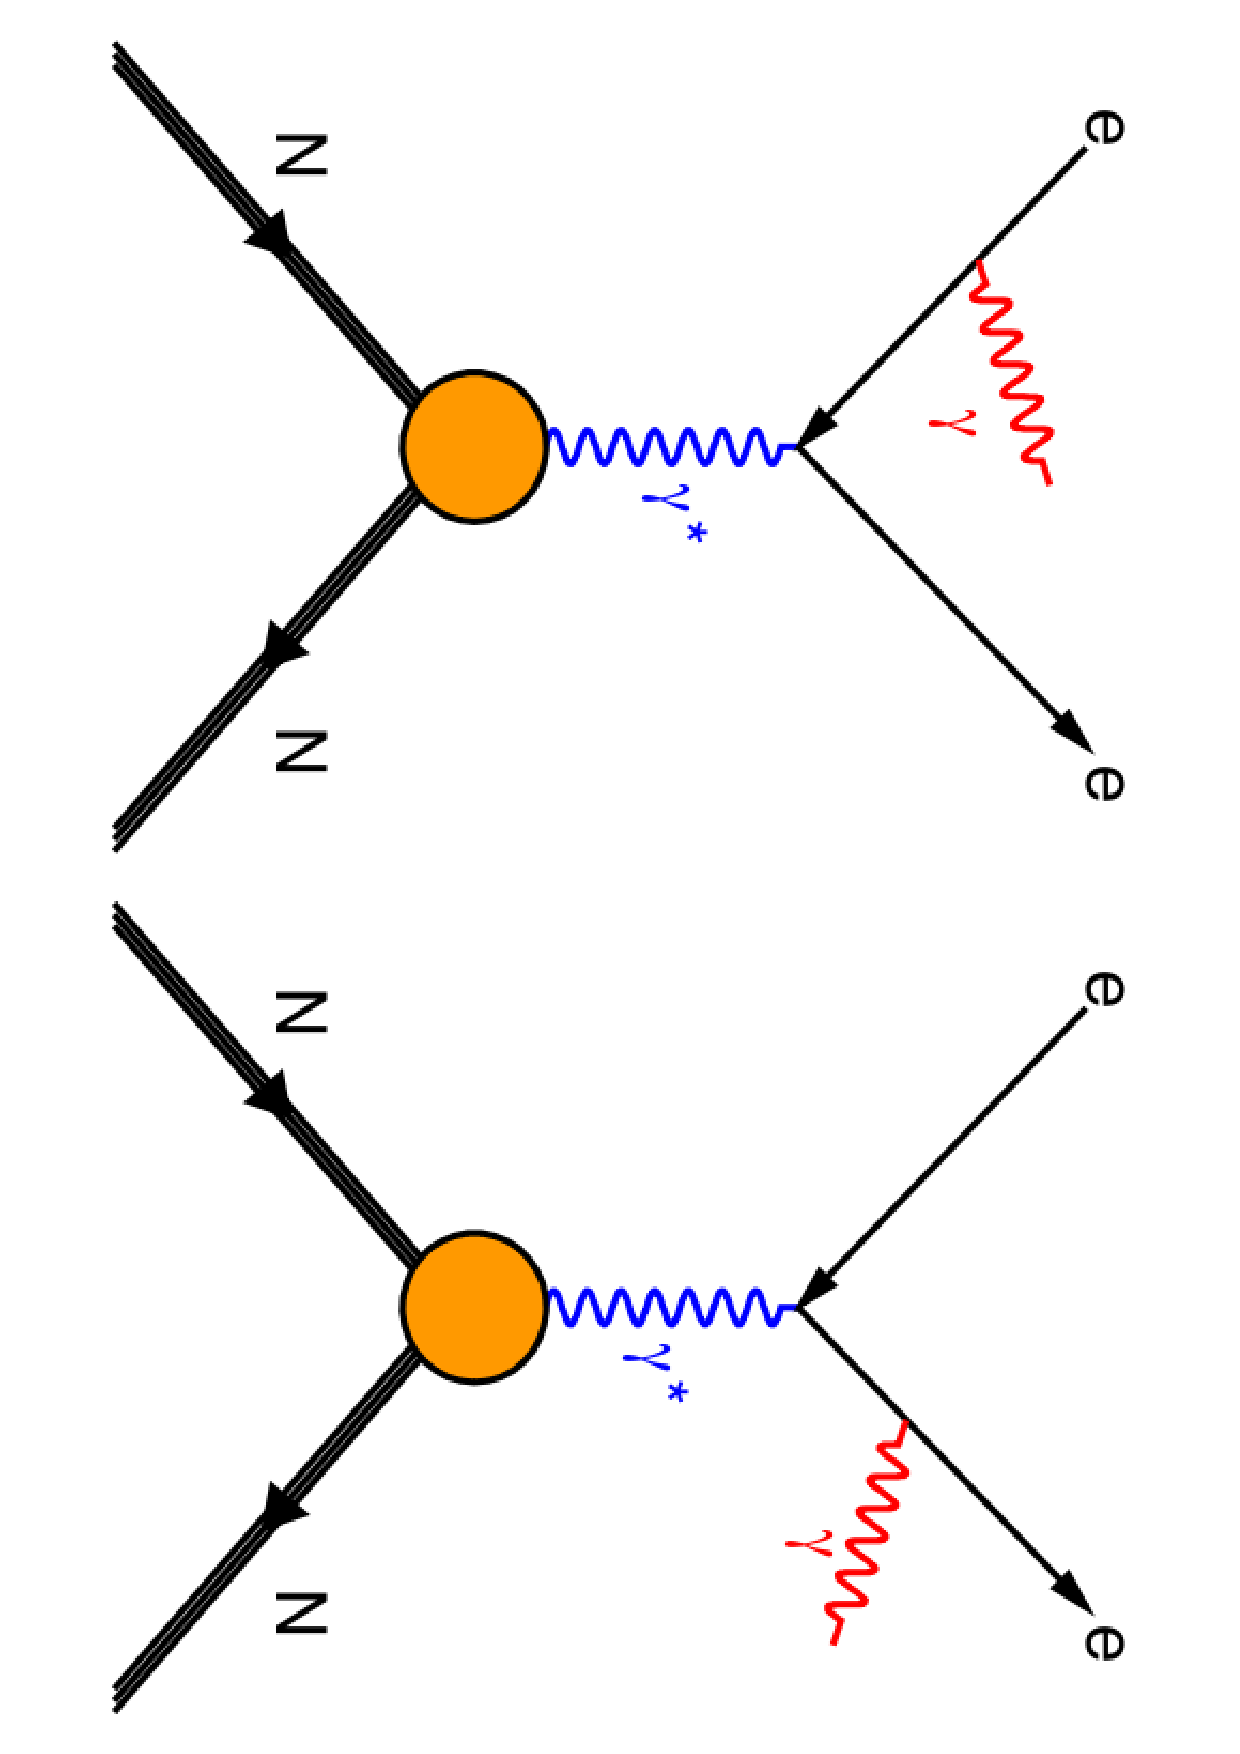
\includegraphics[angle=90,width=0.45\textwidth]{bh_both_edited}}
\caption[DVCS and Bethe Heitler hand bag diagram.]{(a): The leading DVCS process in which an electron/positron ($e$) interacts with a quark in the nucleon
($N$) via a virtual photon ($\gamma^\ast$). The quark is found in the
nucleon with longitudinal momentum fraction $x+\xi$ and emits a real
photon ($\gamma$). The quark is absorbed by the nucleon with
longitudinal momentum fraction $x-\xi$. (b): The leading Bethe-Heitler process, i.e. the emission of a real photon from the incoming or outgoing lepton. This process has the same initial and final states as DVCS.}
\label{spin}
\end{center}
\end{figure}
The BH process is calculable in the QED framework; this process is
dominant at the kinematic conditions of the H{\sc ermes} experiment. The
two processes interfere and the large BH amplitude
amplifies the interference term, which is proportional to the DVCS amplitude. It is through the study of this interference term that useful information for the constraint of certain GPDs can be obtained at H{\sc ermes} kinematic conditions, especially since the interference term is the only part of the squared scattering amplitude that is linear in CFFs~\cite{Bel02b}.

The four-fold differential cross section for the exclusive leptoproduction of real photons
from an unpolarised hydrogen target can be written as \cite{Bel02b}
\begin{center}
\begin{equation}
\frac{\textrm{d}^4\sigma}{\textrm{d}x_{\textrm{B}}\textrm{d}Q^{2}\textrm{d}
|t|\textrm{d}\phi} =
\frac{x_{\textrm{B}}e^{6}}{32(2\pi)^{4} Q^{4}\sqrt{1+\epsilon^{2}}}
|\tau|^{2},
\end{equation}
\end{center}
where $e$ is the elementary
charge, $\epsilon=2x_\textrm{B}\frac{M}{Q}$ with $M$
the target mass, and $\phi$ is the
azimuthal angle between the scattering and production planes \cite{Tre04}.
The {square of the} scattering amplitude $|\tau|^2$ can be written as
\begin{center}
\begin{equation}
|\tau|^{2} = |\tau_{\textrm{BH}}|^{2} +
|\tau_{\textrm{DVCS}}|^{2} + \textrm{I},
\end{equation}
\end{center}
with contributions from the \textrm{BH} process ($\tau_{\textrm{\textrm{BH}}}$),
the DVCS process
($\tau_{\textrm{DVCS}}$) and their interference term (I). These
contributions can be written as
\begin{eqnarray}
 |\tau_{\textrm{BH}}|^{2} &=&
 \frac{K_{\textrm{BH}}}{\mathcal{P}_{1}(\phi)\mathcal{P}_{2}(\phi)} \left(c_{\textrm{unp},0}^{\textrm{BH}} + \sum_{n=1}^2
  c_{\textrm{unp},n}^{\textrm{BH}}\cos(n\phi)\right), \label{e:tbh}\\
|\tau_{\textrm{DVCS}}|^{2} &=&
K_{\textrm{DVCS}}\left(c_{\textrm{unp},0}^{\textrm{DVCS}} +
\sum_{n=1}^2
c_{\textrm{unp},n}^{\textrm{DVCS}}\cos(n\phi) + \lambda\,
s_{\textrm{unp},1}^{\textrm{DVCS}}\sin\phi\right)\,\textrm{and}
\label{e:tdvcs}\\
 \textrm{I} &=& \frac{- e_\ell
K_{\textrm{I}}}{\mathcal{P}_{1}(\phi)\mathcal{P}_{2}(\phi)}\left(c_{\textrm{unp},0}^{\textrm{
I}}+
\sum_{n=1}^3 c_{\textrm{unp},n}^{\textrm{I}}\cos(n\phi) + \lambda \sum_{n=1}^2
s_{\textrm{unp},n}^{\textrm{I}}\sin(n\phi)\right),\label{e:ti}
\end{eqnarray}
where $\mathcal{P}_1(\phi)$ and $\mathcal{P}_2(\phi)$ are the lepton propagators
of the BH process, $\lambda$ is the
helicity of the lepton beam and $e_\ell$ is the sign of the charge of
 the beam lepton.  The
quantities $K_{\textrm{BH}}=1/(x_\textrm{B}^2t(1+\epsilon^2)^2)$,
$K_{\textrm{DVCS}}=1/Q^2$
and $K_{\textrm{I}}=1/(x_{\textrm{B}}yt)$ are kinematic factors, where
$y$ is the fraction of the beam energy carried by the virtual photon in
the target rest frame. A full explanation of the Fourier coefficients [$c_{\textrm{unp},n}^V,s_{\textrm{unp},n}^W$], where V (W) denotes BH, DVCS or I (DVCS or I), can be found in ref.~\cite{Bel02b}.
 
Two sets of asymmetries measured at H{\sc
ermes} with an unpolarised hydrogen target and a polarised electron or positron
beam are considered here:
beam-helicity asymmetries and beam-charge asymmetries. This paper,
like ref.~\cite{Air09}, presents results related to the following asymmetries:
\begin{align}
\hspace{0.5cm}\mathcal{A}^{\textrm{I}}_{\textrm{LU}}(\phi) &\equiv
\frac{(\textrm{d}\sigma(\phi)^{+\rightarrow} -
\textrm{d}\sigma(\phi)^{+\leftarrow}) -
(\textrm{d}\sigma(\phi)^{-\rightarrow}
- \textrm{d}\sigma(\phi)^{-\leftarrow})}{(\textrm{d}\sigma(\phi)^{+\rightarrow}
+
\textrm{d}\sigma(\phi)^{+\leftarrow}) +
(\textrm{d}\sigma(\phi)^{-\rightarrow}
+ \textrm{d}\sigma(\phi)^{-\leftarrow})}&  \nonumber \\
&=\dfrac{-\dfrac{K_{\textrm{I}}}{\mathcal{P}_{1}(\phi)\mathcal{P}_{2}(\phi)}
\displaystyle\sum_{n=1}^2
s_{\textrm{unp},n}^{\textrm{I}}\sin(n\phi)}{\dfrac{K_{\textrm{BH}}}{\mathcal{P}_{1}
(\phi)\mathcal{P}_{
2}(\phi)}
\displaystyle\sum_{n=0}^2
c_{\textrm{unp},n}^{\textrm{BH}}\cos(n\phi) + 
K_{\textrm{DVCS}}\displaystyle\sum_{n=0}^2 c_{\textrm{unp},n}^{\textrm{DVCS}}\cos(n\phi)},& 
\label{e:alui}
\end{align}

\begin{align}
\mathcal{A}^{\textrm{DVCS}}_{\textrm{LU}}(\phi) &\equiv
\frac{(\textrm{d}\sigma(\phi)^{+\rightarrow} +
\textrm{d}\sigma(\phi)^{-\rightarrow}) -
(\textrm{d}\sigma(\phi)^{+\leftarrow} + 
\textrm{d}\sigma(\phi)^{-\leftarrow})}
{(\textrm{d}\sigma(\phi)^{+\rightarrow} +
\textrm{d}\sigma(\phi)^{-\rightarrow}) +
(\textrm{d}\sigma(\phi)^{+\leftarrow}
+ \textrm{d}\sigma(\phi)^{-\leftarrow})}& \nonumber \\[0.4cm]
%\\ \nonumber
&=\dfrac{ K_{\textrm{DVCS}} s_{\textrm{unp},1}^{\textrm{DVCS}}\sin\phi}{\dfrac{K_{\textrm{BH}}}{\mathcal{P}_{1}
(\phi)\mathcal{P}_{2}(\phi)}
\displaystyle\sum_{n=0}^2
c_{\textrm{unp},n}^{\textrm{BH}}\cos(n\phi) + 
K_{\textrm{DVCS}}\displaystyle\sum_{n=0}^2
c_{\textrm{unp},n}^{\textrm{DVCS}}\cos(n\phi)}\, , &
\label{e:aludvcs}
\end{align}

\begin{align}
\hspace{0.5cm}\mathcal{A}_{\textrm{C}}(\phi) &\equiv  
\frac{(\textrm{d}\sigma(\phi)^{+\rightarrow} +
\textrm{d}\sigma(\phi)^{+\leftarrow}) -
(\textrm{d}\sigma(\phi)^{-\rightarrow}
+ \textrm{d}\sigma(\phi)^{-\leftarrow})}{(\textrm{d}\sigma(\phi)^{+\rightarrow}
+
\textrm{d}\sigma(\phi)^{+\leftarrow}) +
(\textrm{d}\sigma(\phi)^{-\rightarrow}
+ \textrm{d}\sigma(\phi)^{-\leftarrow})}&    \nonumber \\
&=\dfrac{{-\dfrac{K_{\textrm{I}}}{\mathcal{P}_{1}(\phi)\mathcal{P}_{2}(\phi)}
\displaystyle\sum_{n=0}^3
c_{\textrm{unp},n}^{\textrm{I}}\cos(n\phi)}}{\dfrac{K_{\textrm{BH}}}{\mathcal{P}_{1}
(\phi)\mathcal{P}_
{2}(\phi)}
\displaystyle\sum_{n=0}^2
c_{\textrm{unp},n}^{\textrm{BH}}\cos(n\phi) + 
K_{\textrm{DVCS}}\displaystyle\sum_{n=0}^2 c_{\textrm{unp},n}^{\textrm{DVCS}}\cos(n\phi)} ,&
\label{e:ac}
\end{align}
where $\textrm{d}\sigma(\phi)^+$ ($\textrm{d}\sigma(\phi)^-$) refers to
the differential cross section with positive (negative) beam charge and
$\textrm{d}\sigma(\phi)^\rightarrow$ ($\textrm{d}\sigma(\phi)^\leftarrow$) refers
to the differential cross section taken with beam spin parallel (anti-parallel) to the
beam momentum.

The $s_{\textrm{unp},n}^{W}$ and $c_{\textrm{unp},n}^{\textrm{W}}$ Fourier
coefficients depend on ``$\mathcal{C}$-functions'' \cite{Bel02b}, each of which is a
combination of CFFs. Contributions to the cross section are suppressed by factors that may be kinematic in nature or due to the twist-level of the GPDs appearing in that contribution. Leading twist is twist-2. Typically, the contribution of a twist-$n$ GPD, and hence the corresponding CFF, is
suppressed by $\mathcal{O}(1/Q^{n-2})$. 

The Fourier coefficients that receive leading-twist contributions are $c_{\textrm{unp},0}^{\textrm{I}}$, $c_{\textrm{unp},1}^{\textrm{I}}$ and $s_{\textrm{unp},1}^{\textrm{I}}$. All of these Fourier coefficients have a dominant contribution from the $\mathcal{C}_{\textrm{unp}}^{\textrm{I}}$-function:
\begin{eqnarray}
c_{\textrm{unp},0}^{\textrm{I}} &\approx&-8(2-y)\frac{(2-y^2)}{(1-y)}K^2\mathfrak{Re}\mathcal{C}_{\textrm{unp}}^{\textrm{I}}\label{eq:c0}
\\
c_{\textrm{unp},1}^{\textrm{I}} &\approx&\,8K(2- 2y + y^{2})\mathfrak{Re}\mathcal{C}_{\textrm{unp}}^{\textrm{I}}\,,\label{eq:c1}
\\
s_{\textrm{unp},1}^{\textrm{I}} &\approx&\,8Ky(2-y)\mathfrak{Im}\mathcal{C}_{\textrm{unp}}^{\textrm{I}}\quad\,. \label{eq:s1}
\end{eqnarray}
The definition of the kinematic factor $K$ is~\cite{Bel02b}:
\begin{equation}
K^2=\frac{t}{Q^2}\Big(1-\frac{t_{\textrm{min}}}{t}\Big)\Big(1-x_{\textrm{B}}\Big)\Big(1-y-\frac{y^2\epsilon^2}{4}\Big)\Big\lbrace\sqrt{1+\epsilon^2}+\frac{4x_{\textrm{B}}(1-x_{\textrm{B}})+\epsilon^2}{4(1-x_{\textrm{B}})}
\frac{t_{\textrm{min}}-t}{Q^2}\Big\rbrace\,.\label{eq:K}
\end{equation} 
The factor of $\Big(1-\frac{t_{\textrm{min}}}{t}\Big)$ implies that amplitudes proportional to these Fourier coefficients vanish as $-t$ approaches its minimum value.
The $\mathcal{C}_{\textrm{unp}}^{\textrm{I}}$-function can be
written
\cite{Bel02b} 
\begin{equation}
 \mathcal{C}_{\textrm{unp}}^{\textrm{I}} = F_{1}\mathcal{H} + \frac{x_{\textrm{B}}}{2-x_{\textrm{B}}}(F_{1}+F_{2})\widetilde{\mathcal{H}} -\frac{t}{4M^{2}}F_{2}\mathcal{E},
\label{Eq_cunp}
\end{equation}
where $F_{1}$ and $F_{2}$ are respectively the Dirac and Pauli form
factors of the nucleon and $\mathcal{H}$, $\widetilde{\mathcal{H}}$ and
$\mathcal{E}$ are CFFs that relate respectively to the GPDs $H$,
$\widetilde{H}$ and $E$.  In H{\sc ermes} kinematic
conditions (where $x_{\textrm{B}}$ and $\frac{-t}{4M^2}$ are of order 0.1), the
contributions of CFFs $\widetilde{\mathcal{H}}$ and $\mathcal{E}$ can be
neglected in eq.~\ref{Eq_cunp} with respect to $\mathcal{H}$ (in first approximation) since they
are kinematically suppressed by an order of magnitude or more.
Hence, the behaviour of
$\mathcal{C}_{\textrm{unp}}^{\textrm{I}}$ is determined by CFF $\mathcal{H}$
and therefore GPD $H$ can be constrained through
measurements of the $\sin\phi$ and $\cos\phi$ terms of the $\mathcal{A}^{\textrm{I}}_{\textrm{LU}}(\phi)$ and $\mathcal{A}_{\textrm{C}}(\phi)$ asymmetries respectively.

Compared to the analysis in ref.~\cite{Air09}, the analysis presented here additionally includes a larger, independent data set taken during the years 2006 and 2007 and makes use of the same missing-mass technique for event selection as was used in ref.~\cite{Air09}. The work covered in this publication further combines the data taken in 1996-2005 with this newer data set to produce the statistically most precise DVCS measurements that will be published by H{\sc ermes}.
